\documentclass[11pt]{article}
\usepackage[a4paper, total={6in, 10in}]{geometry}
\usepackage{graphicx}
\usepackage{amsmath,amsfonts,amssymb}
\usepackage{listings}
\usepackage{booktabs}
\usepackage[T1]{fontenc}
\usepackage{color}
\usepackage{minted}
\usepackage[colorlinks=true, linkcolor=blue, urlcolor=blue, citecolor=blue,
  pdfborder={0 0 255}]{hyperref}
\usepackage{colortbl}
\usepackage{url}
\usepackage{xcolor}
\usepackage{caption}
\usepackage{subcaption}
\usepackage{dirtytalk}
\usepackage[semicolon, round]{natbib}
\usepackage[ruled]{algorithm2e}
\usepackage{multirow}
\usepackage{setspace}
\usepackage{placeins}
\captionsetup[table]{skip=10pt}
\renewcommand{\vec}[1]{\mathbf{#1}}
\SetKwComment{Comment}{$\triangleright$\ }{}
\hypersetup{%
	colorlinks=true,
	linkcolor=blue,
	linkbordercolor={0 0 1}
}

% \renewcommand\lstlistingname{Algorithm}
% \renewcommand\lstlistlistingname{Algorithms}
% \def\lstlistingautorefname{Alg.}

% \lstdefinestyle{Python}{
% 	language        = Python,
% 	frame           = lines,
% 	basicstyle      = \footnotesize,
% 	keywordstyle    = \color{blue},
% 	stringstyle     = \color{green},
% 	commentstyle    = \color{red}\ttfamily
% }

\setlength{\parindent}{0.0in}
\setlength{\parskip}{0.02in}

\newcommand{\argmin}{\mathop{\mathrm{argmin}}}
\newcommand{\argmax}{\mathop{\mathrm{argmax}}}
\newcommand{\minimize}{\mathop{\mathrm{minimize}}}
\newcommand{\maximize}{\mathop{\mathrm{maximize}}}
\newcommand{\st}{\mathop{\mathrm{subject\,\,to}}}
\newcommand{\dist}{\mathop{\mathrm{dist}}}
\newcommand{\norm}[1]{\left\lVert#1\right\rVert}

\renewcommand{\tt}[1]{\texttt{#1}}
% \renewcommand{\vec}[1]{\mathbf{#1}}

\DeclareCaptionType{codelisting}[Listing][List of mytype]
\newenvironment{codeblock}{\captionsetup{type=codelisting}}{}

\def\R{\mathbb{R}}
\def\E{\mathbb{E}}
\def\P{\mathbb{P}}
\def\S{\mathbb{S}}
\def\Cov{\mathrm{Cov}}
\def\Var{\mathrm{Var}}
\def\half{\frac{1}{2}}
\def\quat{\frac{1}{4}}
\def\sign{\mathrm{sign}}
\def\supp{\mathrm{supp}}
\def\th{\mathrm{th}}
\def\tr{\mathrm{tr}}
\def\dim{\mathrm{dim}}
\def\dom{\mathrm{dom}}
\def\th{$^{\mathrm{th}}$}

\title{EE2003 Assignment 3 \vspace{-1em}}
\author{Niranjan A. Kartha, EE21B095\vspace{-3em}}
\date{}

\begin{document}
\maketitle
\section{Question 1 (Problem 2)}
With both architectures, I have attached code written in a way that minimizes and tries to maximize the number of data hazards.

In the minimum-hazard case, I have been able to eliminate all data hazards, and so forwarding does not make a difference in the number of clock cycles taken.

All the below cases output the 15$^{\text{th}}$ Fibonacci number as 610.

\subsection{Flushing delay slots}
\subsubsection{With hazard-free code}
\begin{codeblock}
\inputminted[breaklines,
 mathescape,
 linenos,
 numbersep=5pt,
 frame=single,
 xleftmargin=0pt]{asm}{q1/fib-nobdex.S}
\end{codeblock}

The above code has no hazards, so the pipeline does not stall, with or without forwarding.

\begin{figure}[H]
\begin{subfigure}{.5\textwidth}
  \centering
  
\includegraphics[width=\linewidth]{q1/nox/good/full-91.png}
\end{subfigure}
\begin{subfigure}{.5\textwidth}
  \centering
  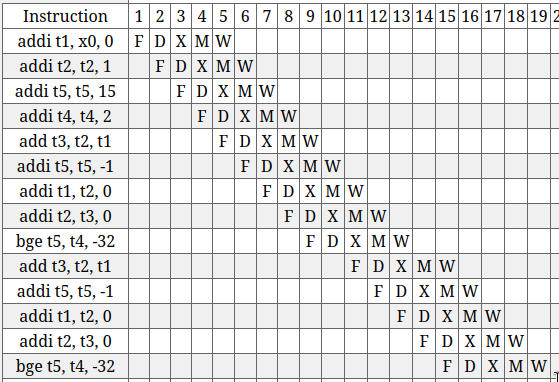
\includegraphics[width=\linewidth]{q1/nox/good/loop.png}
\end{subfigure}
\caption{Execution completes in 91 cycles}
\end{figure}

\newpage

\subsubsection{Code with hazards}
\begin{codeblock}
\inputminted[breaklines,
 mathescape,
 linenos,
 numbersep=5pt,
 frame=single,
 xleftmargin=0pt]{asm}{q1/fib-nobdex-bad.S}
\end{codeblock}
The above code has been written to maximize hazards. Line 6 has a RAW hazard with line 4. Line 8 has a RAW hazard with line 6. Line 10 has a RAW hazard with line 9.

\begin{figure}[H]
\begin{subfigure}{.5\textwidth}
  \centering
  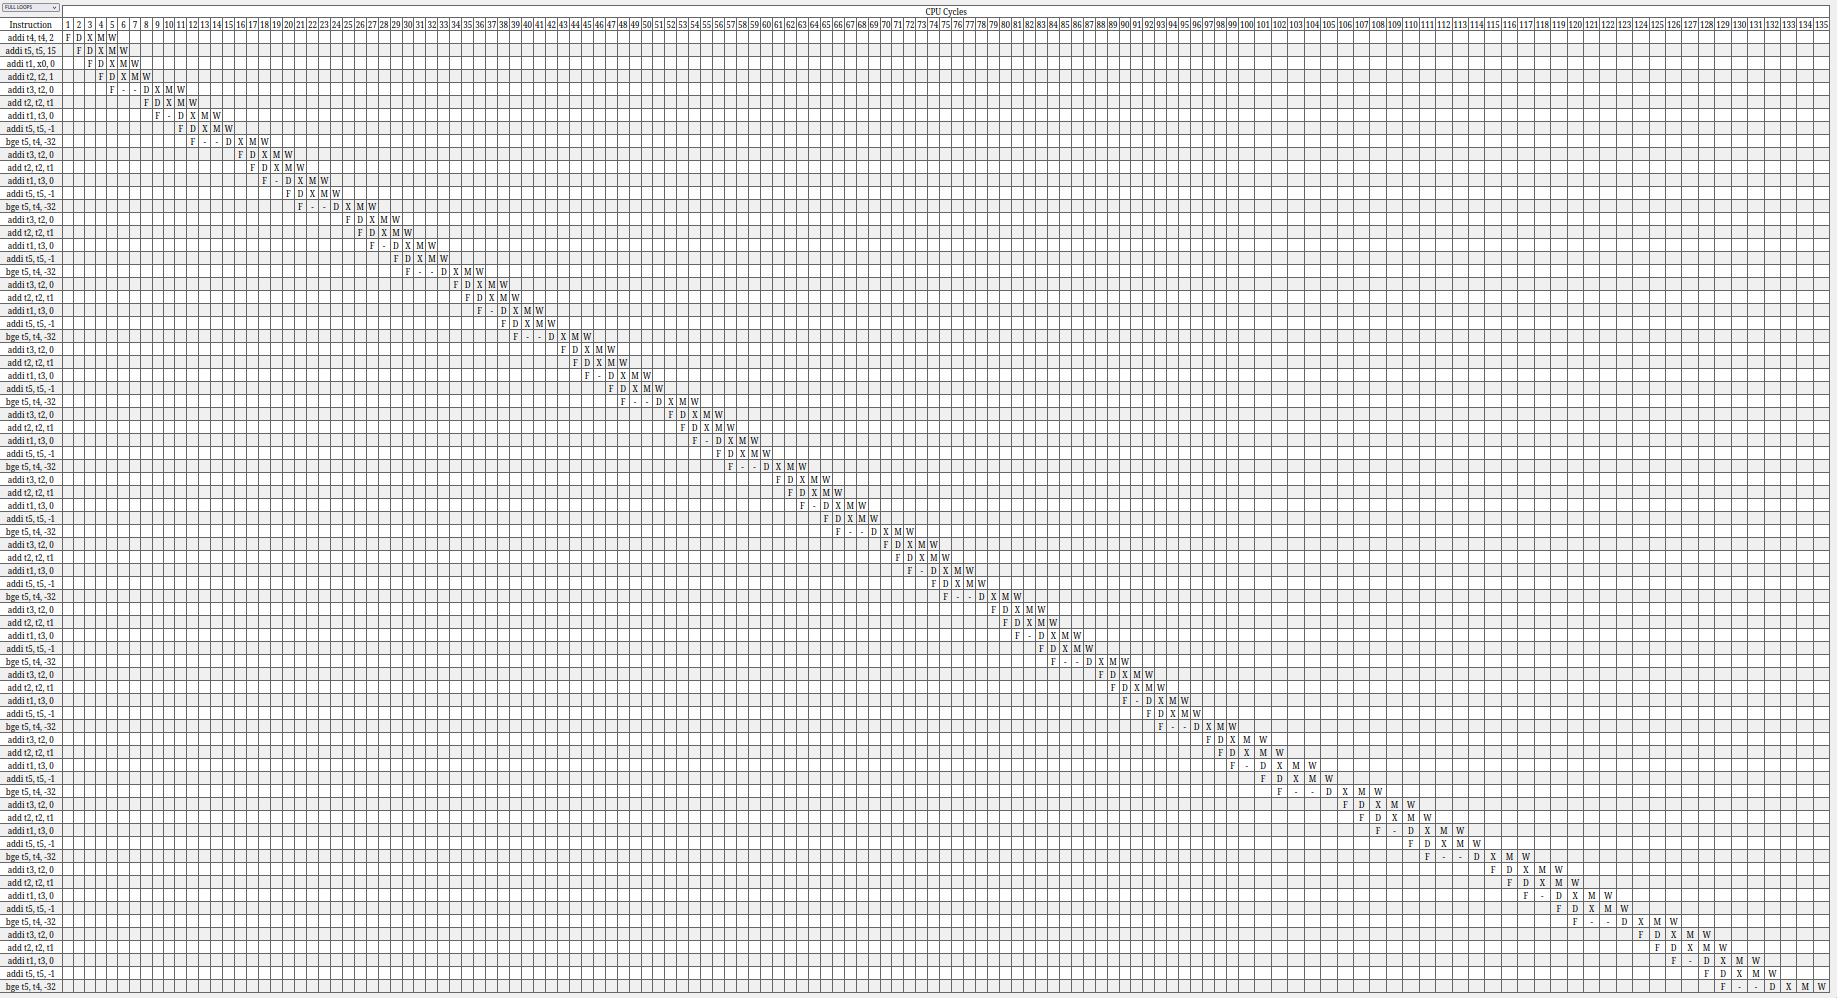
\includegraphics[width=\linewidth]{q1/nox/bad/nof-135.png}
\end{subfigure}
\begin{subfigure}{.5\textwidth}
  \centering
  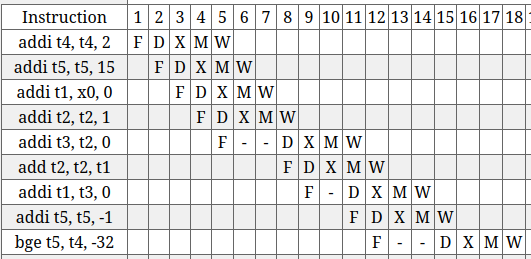
\includegraphics[width=\linewidth]{q1/nox/bad/nof-loop.png}
\end{subfigure}
\caption{Without forwarding, takes 135 cycles}
\end{figure}

\begin{figure}[H]
\begin{subfigure}{.5\textwidth}
  \centering
  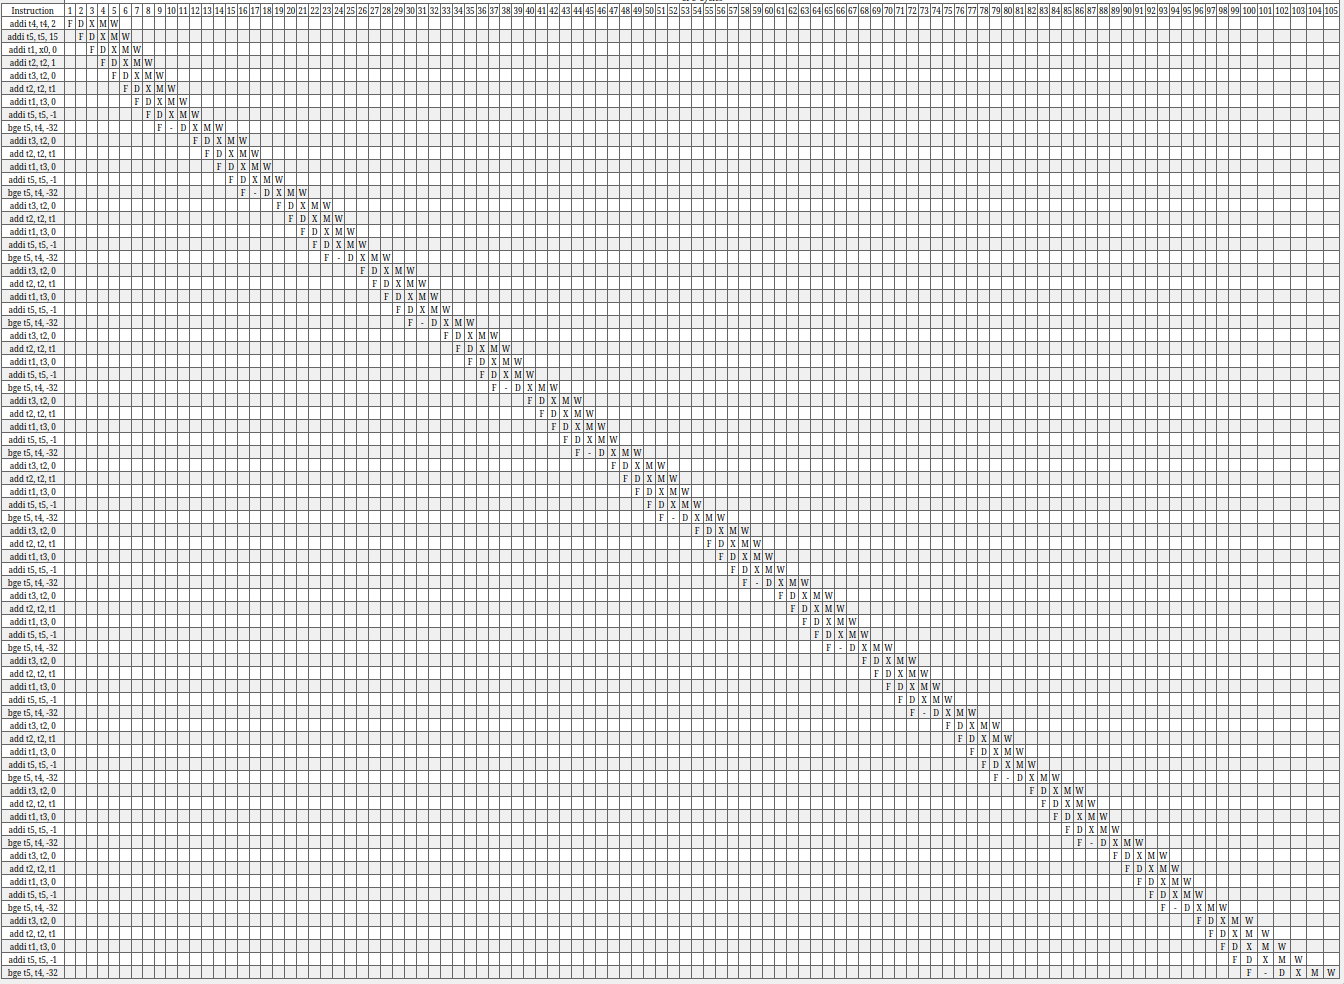
\includegraphics[width=\linewidth]{q1/nox/bad/f-105.png}
\end{subfigure}
\begin{subfigure}{.5\textwidth}
  \centering
  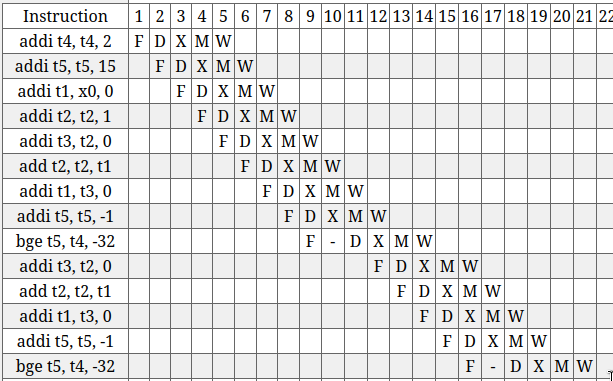
\includegraphics[width=\linewidth]{q1/nox/bad/f-loop.png}
\end{subfigure}
\caption{With forwarding, takes 105 cycles}
\end{figure}

Forwarding does not completely fix the RAW hazard right before the branch.

\newpage

\subsection{Executing delay slots}
If we execute an instruction in the branch delay slot, we can do more useful work while the branch address is being calculated.

\subsubsection{With hazard-free code}
\begin{codeblock}
\inputminted[breaklines,
 mathescape,
 linenos,
 numbersep=5pt,
 frame=single,
 xleftmargin=0pt]{asm}{q1/fib-bdex.S}
\end{codeblock}

The above code has no hazards, so the pipeline does not stall, with or without forwarding. Line 11 also gets executed every time line 10 is encountered.

\begin{figure}[H]
\begin{subfigure}{.5\textwidth}
  \centering
  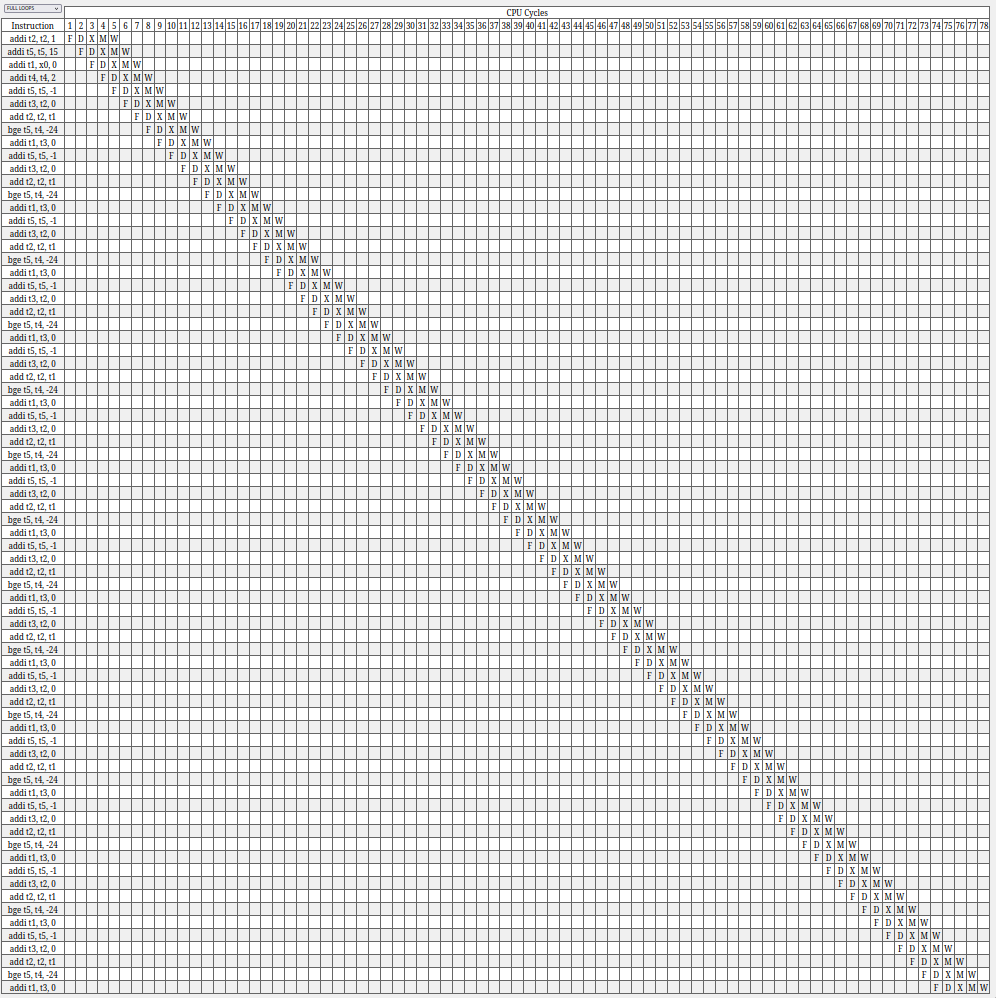
\includegraphics[width=\linewidth]{q1/bex/good/full-78.png}
\end{subfigure}
\begin{subfigure}{.5\textwidth}
  \centering
  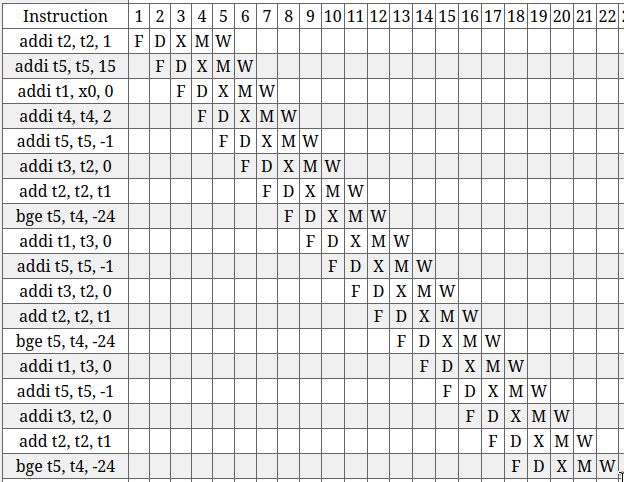
\includegraphics[width=\linewidth]{q1/bex/good/loop.png}
\end{subfigure}
\caption{Execution completes in 78 cycles}
\end{figure}

\newpage

\subsubsection{Code with hazards}
\begin{codeblock}
\inputminted[breaklines,
 mathescape,
 linenos,
 numbersep=5pt,
 frame=single,
 xleftmargin=0pt]{asm}{q1/fib-bdex-bad.S}
\end{codeblock}
The above code has been written to maximize hazards. Line 6 and 7 have a RAW hazard with line 4. Line 9 has a RAW hazard with line 8. Line 6 has a RAW hazard with line 10.

\begin{figure}[H]
\begin{subfigure}{.5\textwidth}
  \centering
  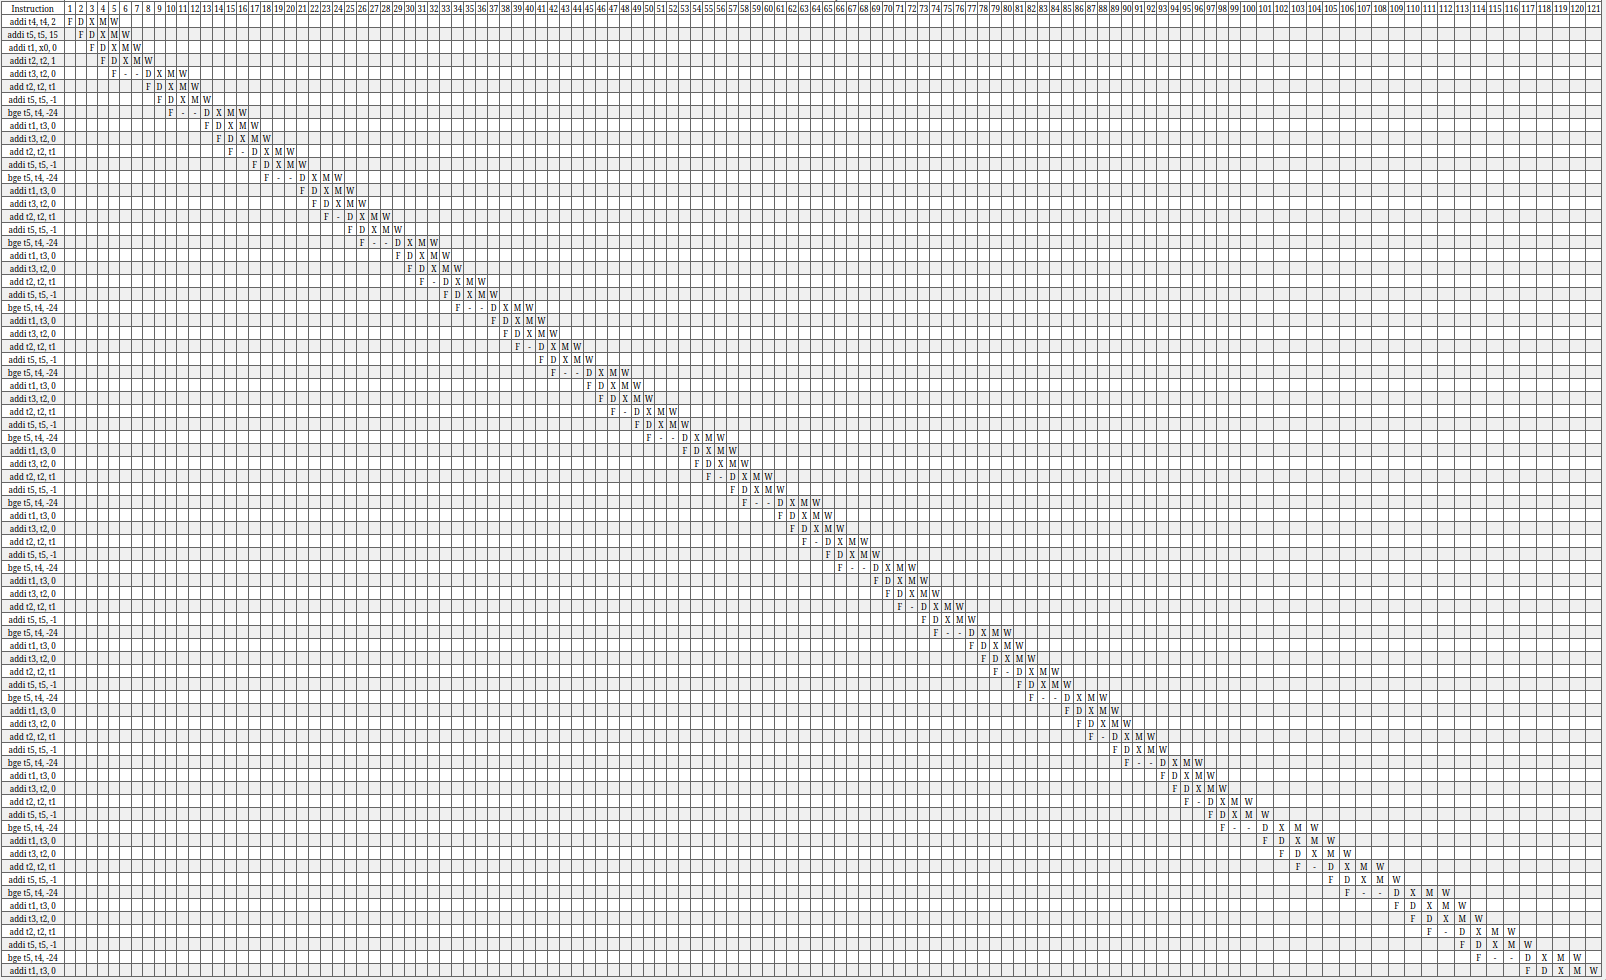
\includegraphics[width=\linewidth]{q1/bex/bad/nof-121.png}
\end{subfigure}
\begin{subfigure}{.5\textwidth}
  \centering
  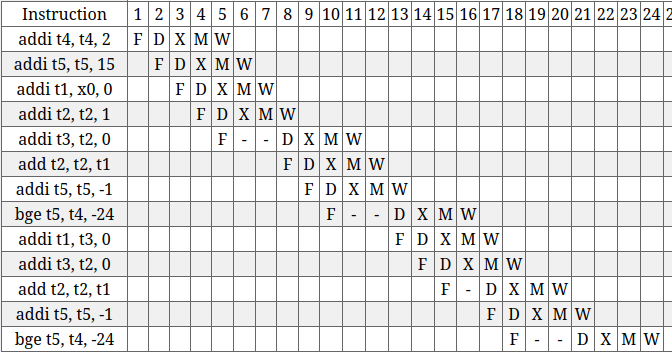
\includegraphics[width=\linewidth]{q1/bex/bad/nof-loop.png}
\end{subfigure}
\caption{Without forwarding, takes 121 cycles}
\end{figure}

\begin{figure}[H]
\begin{subfigure}{.5\textwidth}
  \centering
  
\includegraphics[width=\linewidth]{q1/bex/bad/f-92.png}
\end{subfigure}
\begin{subfigure}{.5\textwidth}
  \centering
  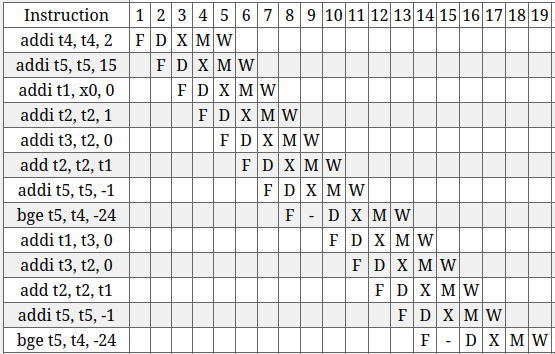
\includegraphics[width=\linewidth]{q1/bex/bad/f-loop.png}
\end{subfigure}
\caption{With forwarding, takes 92 cycles}
\end{figure}

Forwarding does not completely fix the RAW hazard right before the branch.

\newpage

\subsection{Conclusion}
Even with the same instructions being executed, the order in which they are specified is very important for the performance of the program. Instructions need to be written in a way to minimize hazards.

In the above experiments, even with advanced architectural features such as forwarding, code written with care to avoid hazards is always able to outperform code with many hazards.

\section{Question 2 (Dataset 2)}
For the \texttt{matrixmulti.riscv} dataset, these were the results:
\begin{table}[H]
    \centering
    \begin{tabular}{|c|c|c|c|}
    \hline
    \textbf{Strategy} & \textbf{CPI} & \textbf{Control Hazards} & \textbf{Data Hazards} \\
    \hline
    AT & 1.4395 & 29662 & 105128 \\
    NT & 1.4139 & 40678 & 110957 \\
    BTFNT & 1.3893 & 29258 & 110841 \\
    BPB & 1.4129 & 29482 & 108238 \\
    \hline
    \end{tabular}
    \label{tab:q1values}
\end{table}

\subsection*{Observations}
Matrix multiplication involves a lot of looping, and so the results are as follows:
\begin{itemize}
  \item AT performs poorly because it mispredicts almost every time a loop performs an iteration.
  \item NT performs well, since it fits backward branches in loops well.
  \item BPB performs well, since it is able to learn how branches behave.
  \item BTFNT performs best, since this is the natural way that branches tend to behave in normal use-cases. It does not need to waste branch mispredictions in trying to learn how a branch will behave.
\end{itemize}

\end{document}
